% TeX root = ../Main.tex

% First argument to \section is the title that will go in the table of contents. Second argument is the title that will be printed on the page.
\section[Lecture 1 -- {\it Alpha Particle}]{Lecture 1 (1/21)}

\subsection{Alpha Decay}
Geiger and Nutall noticed a trend where a slight difference in the disintegration energies or Q-values
of radioactive samples brought about a huge difference in the half life. $\ce{^{232}He}$(1.4 X 10” y; Q = 4.08 MeV) $\ce{^{218}Th}$(1.0 X l o p 7 s; Q = 9.85 MeV)
so a factor of 2 in energy brings about a factor of $10^24$ in half life. 
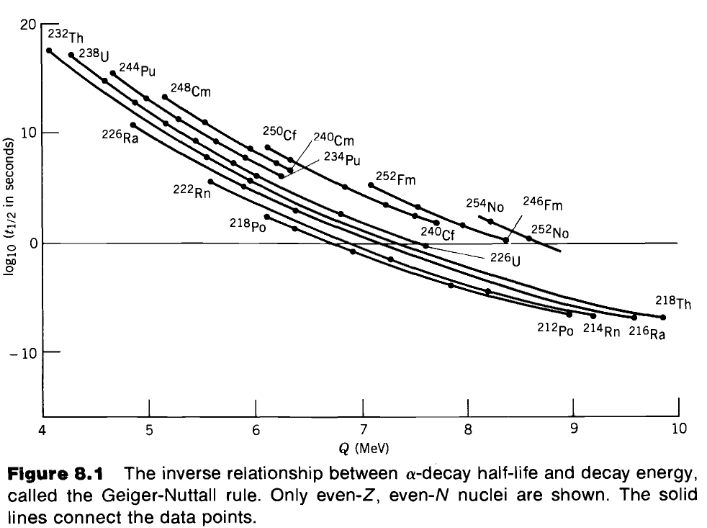
\includegraphics[width=\linewidth]{Geiger-Nutall_plot.png}
Even-odd, odd-even and odd-odd nuclei also show the same trend as the above even-even nuclei but 
don't result in lines as smooth. Their periods are 2-1000 times larger than the even-even types.

General features of the above plot can be explained by the Quantum Mechanical theory developed simultaneously 
in 1928 by Gamov and Churney and Condon. In this theory, the $\alpha$ particle assumed to be formed inside
the nucleus before emission. 

Do keep in mind that just because this theory can explain nuclear behaviour
does not mean that $\alpha$ particle really is formed in the nucleus before emission, it just means that 
it behaves as if that was the case.

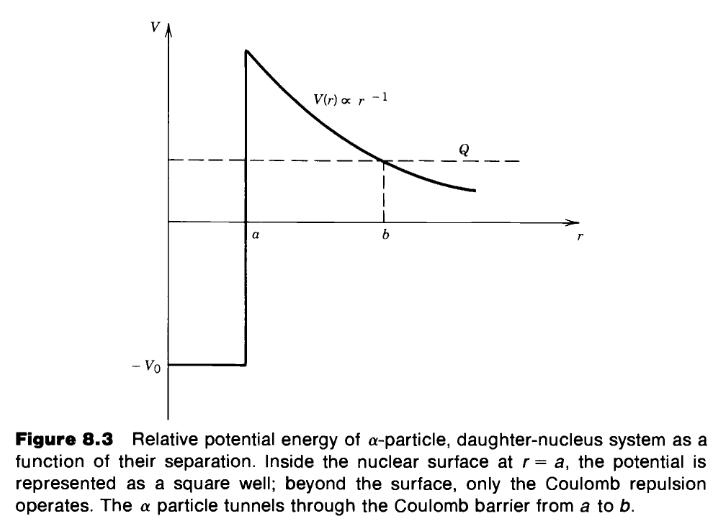
\includegraphics[width=\linewidth]{alpha_potential.png}

The above is a plot of potential between $\alpha$ particle and residual nuclei($V_{0}$) against the distances 
between their centres(r). The horizontal dotted line is the disintegration energy Q and 'a' can be taken as the sum of radii of $\alpha$ particle and residual nucleus.
There are three areas of interest, for r<a, we are inside the nucleus, with a potential well of $-V_{0}$, classically the particle can move 
here with potential of $Q+V_{0}$. The shell area a<r<b forms a potential barrier here as the potential
energy here is higher than the available energy Q. So $\alpha$ particle is not supposed to be able to 
enter this area through either side, classically that is. b<r is the classically allowed area outside the barrier.
According to classical mechanics then, $\alpha$ decay should not be possible at all, but quantum mechanically, there 
is a small possibility of an event called 'tunneling' to occur where the $\alpha$ particle gets to the 
other side despite the barrier. 

The probability of this event is extremely low, that's why $\alpha$ unstable 
nuclei don't just decay all the time. For example, in $\ce{^{238}U}$, the $\alpha$ particle has to "hit" the 
potential barrier approximately $10^28$ times before it can get out. The same principle follows in the 
case of an incident particle from the other side of the barrier(with lower energy than the potential well of course). 
Fusion reactions, such as those responsible for the energy released in stars are analyzed using the barrier penetration approach.

The disintegration constant of an $\alpha$ emitter in one-body theory is given by 
$$\lambda=fP$$
Where $f$ is the frequency of the alpha particle "hitting" the barrier and $P$ is the probability of transmission through the barrier.




\subsection{Second subsection}